\pdfminorversion=7
\documentclass[]{interact}

\usepackage[T1]{fontenc}
\usepackage[utf8]{inputenc}
\usepackage{epstopdf}
\usepackage{subfigure}
\usepackage{natbib}
\usepackage{array}
\usepackage{tabularx}
\usepackage{hyperref}
\hypersetup{hidelinks}
\bibpunct[, ]{(}{)}{;}{a}{}{,}
\renewcommand{\bibfont}{\fontsize{10}{12}\selectfont}

\theoremstyle{plain}
\newtheorem{theorem}{Theorem}[section]
\newtheorem{lemma}[theorem]{Lemma}
\newtheorem{corollary}[theorem]{Corollary}
\newtheorem{proposition}[theorem]{Proposition}
\theoremstyle{definition}
\newtheorem{definition}[theorem]{Definition}
\newtheorem{example}[theorem]{Example}
\theoremstyle{remark}
\newtheorem{remark}{Remark}
\newtheorem{notation}{Notation}


% Revision v2: keep figures proportional and prevent float-page vertical spreading.
\usepackage{lmodern}
\usepackage{xurl}
\usepackage{placeins}
\newcolumntype{Y}{>{\raggedright\arraybackslash}X}
\emergencystretch=2em
\makeatletter
\setlength{\@fptop}{0pt}
\setlength{\@fpsep}{12pt}
\setlength{\@fpbot}{0pt plus 1fil}
\makeatother
\renewcommand{\topfraction}{0.95}
\renewcommand{\bottomfraction}{0.95}
\renewcommand{\textfraction}{0.05}
\renewcommand{\floatpagefraction}{0.80}
\setcounter{topnumber}{3}
\setcounter{totalnumber}{5}
\setlength{\textfloatsep}{12pt plus 2pt minus 2pt}
\setlength{\floatsep}{12pt plus 2pt minus 2pt}

\begin{document}

\title{A Ground--Low-Altitude Mobility Manager for Service Reconfiguration under Disruptions}

\author{
\name{An Xu\textsuperscript{a} and 
Yunfei Yin\textsuperscript{a}\thanks{CONTACT Yunfei Yin. Email: yunfeiyin@hit.edu.cn. 
An Xu. Email: AnX.RTL2324@tum-asia.edu.sg}}
\affil{\textsuperscript{a}School of Transportation Science and Engineering, 
Harbin Institute of Technology, Harbin 150090, China}
}

\maketitle

\begin{abstract}
While integrating low-altitude resources offers a promising avenue for ground transport resilience, simply deploying aircraft does not guarantee that disrupted time-critical services will meet their deadlines. We demonstrate that effective service recovery requires dynamic, time-aware cross-modal coordination rather than mere physical path restoration. To address this, we propose a Ground-Low-Altitude Mobility Manager—a service-level supervisory architecture that converts joint ground-air observations into a shared executable candidate interface. This framework allows replaceable supervisory policies, including fixed-objective heuristics and Large Language Model (LLM)-based agents, to evaluate feasible interventions against incumbent-service costs and remaining temporal margins. Through SUMO-BlueSky co-simulation across distinct urban morphologies, our experiments reveal a critical operational trade-off: faster emergency air transport often requires preempting occupied resources, displacing existing services even when ground fallback remains timely. While both heuristic and LLM policies halved emergency deadline violations (from 33.33\% to 16.67\%) in a meshed urban network, they exhibited markedly different incumbent-service damage (0.058 versus 0.133 damaged services per run, respectively). Furthermore, we show that explicit candidate-information support significantly alters LLM choices, and that delayed execution can consume the remaining margin. Ultimately, this study highlights that realized transport resilience depends not just on available air capacity, but on securing timely, service-aware interventions.
\end{abstract}

\begin{keywords}
ground--low-altitude mobility; service reconfiguration; disruption management; supervisory control; transport resilience; network morphology.
\end{keywords}

\section{Introduction}

Restoring network connectivity does not necessarily restore transport service. An urgent mission may still have a road route but no longer have enough time to meet its deadline. A useful response must preserve on-time completion within the remaining service margin. Reassigning a vehicle can rescue that mission while interrupting another service. Disruption management must therefore consider both deadline compliance and how service losses are distributed, consistent with performance-based transport resilience assessment. \citep{ref1}

Low-altitude resources offer a way around disrupted ground links. Their value depends on where they are, which tasks they can serve and whether they are already occupied. Using a faster aircraft may require preempting an incumbent service even when continued ground transport would meet the deadline. Communication loss, degraded navigation or an unavailable landing site can also remove the air alternative after dispatch. The management problem is to select and execute useful cross-modal interventions as resources and deadlines change.

Multimodal recovery and Resilience as a Service coordinate heterogeneous replacement services, while dynamic fleet management and truck--drone routing address changing assignments and synchronization. \citep{ref4,ref19,ref20,ref21,ref22} Constrained-execution architectures distinguish a proposed action from permission to apply it. \citep{ref8} We bring these ideas together for supervisory service reconfiguration, using a failure-prone air layer to support disrupted ground services. A common interface describes feasible interventions and their consequences. It allows us to compare selection policies under controlled conditions and trace why a feasible replacement can still arrive too late.

We propose the \textbf{Ground--Low-Altitude Mobility Manager} (hereafter, the Manager). It connects joint state observations, deterministic candidate generation, replaceable supervisory selection and common execution checks. The \textbf{shared executable candidate interface} reports resource compatibility, legality, estimated completion and the incumbent service each option would displace. The supervisor selects one intervention. The executor normalizes and validates the proposal, then issues it or queues it for revalidation. Local contingencies operate independently. Here, global state means the joint state of one modeled study area. Ground service uses a SUMO corridor ETA timer; air transport evolves in BlueSky.

We make three contributions. First, we develop a supervisory architecture for ground--air service reconfiguration that specifies how observations, selection and execution interact. Second, we provide the shared candidate interface and compare ground-only, air-first, fixed-objective heuristic and LLM-candidate policies. Third, we quantify how surviving alternatives, service trade-offs and observation--execution timing affect transport outcomes. Selective air support can reduce missed deadlines while displacing incumbent services. A restored path can still finish late, and delayed execution can allow a new command to replace the selected action. Figure~\ref{fig:fig01} links these findings to E1 selective support, E2 single air failure, E3 compound disturbance and E4 timing and input burden.

\begin{figure}[!htbp]
\centering
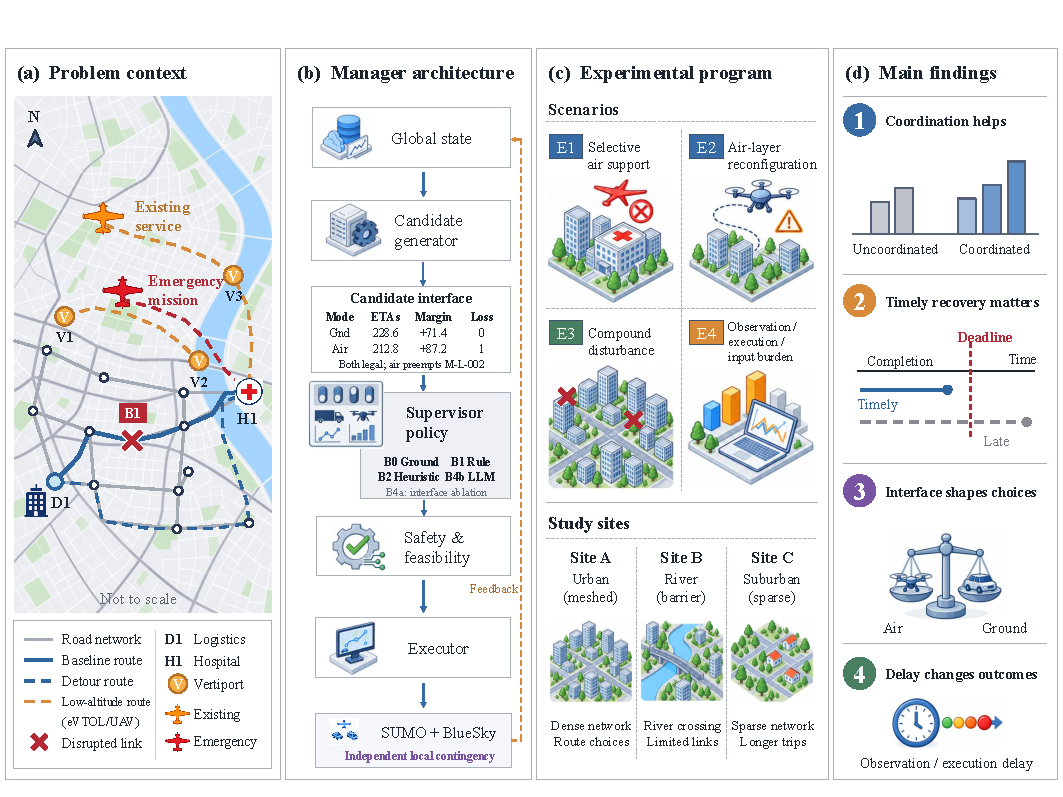
\includegraphics[width=\textwidth]{figures/fig01.pdf}
\caption{Overview of the Ground-Low-Altitude Mobility Manager. (a) Schematic service network with logistics D1, hospital H1, landing nodes V1--V3, ground and low-altitude routes, and a disrupted link B1. The schematic map is not to scale; map B1 is distinct from policy B1. (b) Shared candidate facts connect replaceable supervisory policies to modeled feasibility checks and execution. B0/B1/B2/B4b are primary policies; B4a is an E1 interface ablation. (c) E1 examines selective air support, E2 air-layer reconfiguration, E3 compound disturbance and E4 observation, execution and input burden. E1--E3 use sites A--C; E4 uses A. (d) Conceptual findings express conditional coordination benefit, timely recovery, interface-dependent choices and delay effects. The interface effect is strongest at A. Illustrations are schematic; symbols and bars are qualitative, not measured outcomes.}
\label{fig:fig01}
\end{figure}

\FloatBarrier
\section{Related work}

\subsection{Disruption management across transport services}

Transport vulnerability and resilience research connects component disruptions to changes in system performance. Mattsson and Jenelius distinguish the related concepts, while Jenelius and Mattsson explain how network vulnerability measures can be implemented. \citep{ref1}, \citep{ref2} Cats and Jenelius show why partial capacity degradation also matters for public transport performance. \citep{ref3} These studies motivate evaluating service completion and deadline compliance alongside the existence of an alternative route.

Operational responses can propagate between transport services. Lai and Leung study real-time public transit rescheduling under disruption. \citep{ref5} Yap et al. couple train rescheduling with dynamic passenger assignment to represent disruption propagation into urban tram and bus networks. \citep{ref19} Their framework makes effects outside the initially disrupted layer part of the response assessment. Here, incumbent-service damage provides a narrower service-level account of such consequences, without modeling passenger redistribution across a public transport network.

Jaber et al. formulate Resilience as a Service through resource allocation among buses, taxis and automated vans that can bridge disrupted rail services. \citep{ref20} Their work provides a close precedent for coordinating heterogeneous replacement services. Our setting adds a failure-prone air layer. We compare interchangeable supervisory policies through the shared candidate interface and examine how their executed interventions affect service.

\subsection{Dynamic fleet management and ground--air coordination}

Dynamic vehicle routing addresses assignment and routing decisions as operational information changes. \citep{ref4} Ground--air coordination introduces resource synchronization: the flying sidekick traveling salesman problem jointly plans truck and drone movements for parcel delivery. \citep{ref6} Meng et al. incorporate stochastic truck travel times and soft time windows, using rolling-horizon recourse to update truck waiting times during execution. \citep{ref21} Their work illustrates that timing and synchronization are substantive transport decisions, beyond selecting the nominally fastest mode.

At the network level, Wollenstein-Betech et al. jointly optimize intermodal vehicle routing and rebalancing while accounting for congestion generated by vehicle flows. \citep{ref22} Our model selects an intervention for an actionable service and represents ground transport through a shared corridor travel-time proxy. It does not optimize network-wide routing flows or truck--drone launch-and-retrieval tours. We compare how policies select, preserve or replace services as modeled feasibility changes. B2 ranks candidates one step at a time using an explicit preference between faster completion and preserving incumbent service.

\subsection{Supervisory selection and constrained execution}

Urban air mobility concepts distinguish vehicle operations, operating locations and supporting management services. \citep{ref7} More generally, control architectures can separate a proposed action from the mechanism permitting execution. Wabersich and Zeilinger's predictive safety filter exemplifies this separation under a specific constrained-control formulation. \citep{ref8} We adopt the proposal--execution separation and implement transport-specific deterministic rule checks.

The candidate generator reports common feasibility, completion-time and incumbent-service facts before the supervisor selects an action. The executor then checks the chosen action against the current state. Policies can therefore express different preferences while using the same rules for deriving information and checking execution. This separation also lets us trace what happens between a feasible proposal and the intervention that executes.

\subsection{Language models and the comparison addressed here}

SayCan connects language-based choices to executable robotic capabilities, while LLMLight applies language-based decisions to traffic signal control. \citep{ref9,ref10} These studies motivate an LLM as one implementation of the supervisory policy. Long-context research also distinguishes information availability from effective use. \citep{ref11}

We ask how policies use the common service-management contract and when their executed interventions protect service. The B4a--B4b comparison separately tests explicit candidate-information support within the same LLM implementation. The ablation removes derived per-candidate facts as well as their presentation, so it tests information support rather than table formatting alone.

\section{Problem formulation}

\subsection{Ground--low-altitude service system}

Let the ground network be a directed graph $G^g=(V^g,E^g)$. The low-altitude layer contains aircraft, operating sites, assignments, routes and active restrictions. Time advances in discrete simulation steps. At time $t$, the combined service state is

\begin{equation*}
S_t=(G_t,A_t,I_t,M_t,E_t), \tag{1}
\end{equation*}

where $G_t$ contains ground connectivity and travel-time estimates, and $A_t$ contains aircraft states. $I_t$ describes landing infrastructure and operating restrictions; $M_t$ is the mission registry. $E_t$ records currently represented disturbances and recent events. A mission $m$ has a release time $r_m$, absolute deadline $d_m$, origin, destination, service type, priority $p_m$, state and configured penalties. An aircraft has a role, assignment status, position, remaining endurance, landing compatibility and commandability.

A disruption can change ground travel time, interrupt a selected air chain, remove an aircraft from supervisory control or eliminate a landing option. The same external event can affect policies differently because their earlier assignments determine which missions are exposed. Cross-modal reconfiguration changes a task's resource or transport mode, or changes how an existing operation continues. It can improve an emergency's outcome while interrupting or otherwise changing the state of an incumbent service.

The supervisor receives an observation

\begin{equation*}
\widehat S_t=\mathcal O_t(S_{0:t}),\qquad \tau(t)\le t, \tag{2}
\end{equation*}

where $\mathcal O_t$ incorporates snapshot sampling and event ordering, and $\tau(t)$ is the snapshot timestamp. Snapshot age $t-\tau(t)$ helps describe visibility, but it does not identify every visible event. An event injected after a snapshot is absent even if both occur in the same simulation second. This distinction matters in the observation-scheduling experiment.

\subsection{Candidate information and feasible alternatives}

A deterministic mapping $\Phi$ constructs the candidate information interface,

\begin{equation*}
\mathcal I_t=\Phi(\widehat S_t),\qquad
\mathcal C_{m,t}=\{c\in\mathcal I_{m,t}:\operatorname{legal}(c\mid\widehat S_t)=1\}. \tag{3}
\end{equation*}

$\mathcal I_{m,t}$ contains the records for mission $m$; $\mathcal C_{m,t}$ is the subset marked legal. The interface also keeps rejected resource records and their rejection reasons. Each candidate record identifies the mission, resource, transport mode and implied action. It reports estimated remaining completion duration $\widehat\eta_c$, feasibility status, endurance information, destination conditions and any incumbent service that would be displaced.

Air feasibility depends on availability, mission compatibility, commandability, battery/endurance conditions, landing-site compatibility and modeled restrictions. Reassignment of an occupied aircraft requires an explicitly reassignable incumbent mission with strictly lower priority than the target. A ground candidate is available when the mission permits ground fallback and a travel-time estimate is present. These candidates represent the alternatives generated by the implemented service model; they do not enumerate every possible route or future schedule.

The interface contains no B2 objective score, optimizer selection or manager-specific recommended action. It does, however, reflect shared modeling choices: priority constraints, travel-time approximations and the organization of multi-mission records. Here, manager-agnostic means that policies use the same generation rules and facts at a given state. It does not mean that the representation is free of operational assumptions. After policies take different actions, their states and candidate sets can also differ.

\subsection{Supervisory actions and execution-time constraints}

At a decision epoch, policy $k$ proposes one structured intervention:

\begin{equation*}
a_t^{\mathrm{prop}}=\pi_k(\widehat S_t,\mathcal I_t),\qquad
k\in\{\mathrm{B0,B1,B2,B4b}\}. \tag{4}
\end{equation*}

The action contract includes assignment and reassignment actions, route or destination changes, ground fallback, and management responses such as delay or no action. A proposal need not correspond to selecting an aircraft. In particular, B0 restricts cross-modal emergency support to the ground alternative.

Let $t_e=t+\delta_{\mathrm{exec}}$ be a proposal's scheduled execution time. Let $Q(a,t_e)$ indicate that the proposal remains the active command version for the relevant task, and let $\Gamma(a,S_{t_e})$ denote the semantic and feasibility check using the current execution state. Abstracting the action-specific normalization performed by the implementation, the executed intervention is

\begin{equation*}
u_{t_e}=\begin{cases}
\operatorname{Executor}(a_t^{\mathrm{prop}},S_{t_e}),
&Q(a_t^{\mathrm{prop}},t_e)=1\land\Gamma(a_t^{\mathrm{prop}},S_{t_e})=1,\\
\varnothing,&\text{otherwise}.
\end{cases} \tag{5}
\end{equation*}

A newer command can supersede a pending proposal; the executor rejects a proposal that fails the current checks. Neither supersession nor rejection means that transport has been completed. The subsequent state follows

\begin{equation*}
S_{t+1}=F(S_t,u_t,e_t,\ell_t), \tag{6}
\end{equation*}

where $e_t$ represents exogenous events and $\ell_t$ represents local contingency responses. This notation describes the implemented supervisory interface and event-driven simulator evolution.

\subsection{Service outcomes and temporal feasibility}

For a completed mission, completion duration and deadline violation are

\begin{equation*}
T_m=c_m-r_m,\qquad V_m=\mathbf1[c_m>d_m], \tag{7}
\end{equation*}

where $c_m$ is the absolute completion time. Completion exactly at the deadline is on time. A useful diagnostic for a candidate at decision time $t$ is its estimated temporal margin,

\begin{equation*}
\sigma_m(c,t)=d_m-t-\delta_{\mathrm{exec}}-\widehat\eta_c,\qquad
\mathcal C^{\mathrm{timely}}_{m,t}=\{c\in\mathcal C_{m,t}:\sigma_m(c,t)\ge0\}. \tag{8}
\end{equation*}

A feasible candidate set may contain no alternative predicted to finish on time. Even a nonnegative estimated margin does not guarantee on-time completion: later failures, queue changes or estimation error can change the outcome. Equation (8) links candidate facts to the decision regimes analyzed in Figure~\ref{fig:fig04}.

We evaluate service resilience through path restoration, deadline compliance, incumbent-service preservation and priority-weighted loss. These outcomes describe complementary aspects of supervisory recovery. They do not measure infrastructure repair or imply that all parts of the transport system have returned to their original operating conditions.

\section{Ground--Low-Altitude Mobility Manager}

\subsection{Global state and closed-loop environment}

The simulation environment couples SUMO for road traffic with BlueSky for aircraft movement. \citep{ref12}, \citep{ref13} A master orchestrator advances both layers in 1 s steps, maintains the service registry, and applies events and accepted interventions. Figure~\ref{fig:fig01}(b) places the replaceable policy within this sequence. Local aircraft contingencies operate independently of supervisory inference.

The snapshot combines road estimates and closures with aircraft assignments, endurance, commandability, landing-site conditions, and mission priorities and deadlines. Ground candidates use the shared D1--H1 corridor ETA, including for eligible missions in the multi-mission interface. When ground fallback executes, the executor queries the current SUMO corridor estimate and schedules completion using the rounded duration. A mission timer records completion; the model does not dispatch and track a separate road vehicle for each fallback mission.

The simulators are coupled through task status and resource assignment. A new air assignment routes the aircraft from its current position through the mission origin to the destination. For an interrupted mission, the candidate route passes through the contingency site V3 before reaching the destination. Preemption detaches the incumbent mission and changes the aircraft's assignment. Local return or diversion continues separately. Replacement dispatch does not require verification that the original payload has arrived at V3. The registry does not model payload custody, unloading, reloading or re-shipment. Ground fallback changes the mission's mode and schedules completion from the live corridor ETA; it uses the proposal ETA only if the live query is unavailable. These rules represent service replacement. Supplementary Section S4 separately examines physical transfer time through an offline sensitivity analysis of the remaining margin.

\begin{center}
\begin{minipage}{0.96\textwidth}
\hrule\vspace{5pt}
\textbf{Algorithm 1. Ground--air supervisory service reconfiguration}
\begin{enumerate}\setlength{\itemsep}{1pt}\setlength{\parskip}{0pt}
\item Initialize both simulators, the mission/resource registry and the observation and pending-command stores.
\item At each simulation step, apply scheduled events. Their local contingency responses run independently of supervisory inference.
\item At an event or periodic decision opportunity, observe the joint state (the latest stored snapshot in E4A); build candidate facts for the actionable mission(s).
\item Select one supervisory intervention using policy $\pi$; normalize missing route/target fields and validate its structure, semantics and modeled feasibility. Log rejected proposals.
\item Issue an accepted intervention immediately, or queue it for $t+\delta_{\rm exec}$. Keep the original due time for an identical pending command; a changed command supersedes the previous one for that mission.
\item After same-time events and their decisions, process due commands: normalize again, refresh state and revalidate. Skip completed effects; on stale rejection request a new decision; otherwise execute.
\item Advance SUMO and BlueSky by 1 s; update mission/resource states, ground completion timers and scheduled observations. Repeat until the horizon.
\end{enumerate}
\vspace{3pt}\hrule
\end{minipage}
\end{center}

Algorithm 1 processes same-time events before pending commands. Ordinary periodic decisions are suppressed while an actionable mission has a pending command; E4A uses its scheduled polling protocol instead. Section 6.6.2 examines how these queue rules affect completion time. Independent local contingencies do not wait for the queue.

\subsection{Candidate generator and shared executable interface}

The candidate generator computes candidate facts from the observed global state. The shared executable candidate interface defines the fields and action semantics available to the supervisor. It makes air and ground alternatives comparable without recommending a selection. All candidates use the same convention for estimated remaining completion duration. Air estimates combine modeled route geometry, role-specific cruise speeds and dispatch overhead; ground candidates use the common fallback estimate. The interface also reports estimated absolute completion time, remaining deadline margin and whether preemption would interrupt an incumbent service. The supervisor uses these estimates to choose an intervention. At execution, the executor refreshes operational quantities from the environment and applies deterministic checks against the modeled constraints.

\begin{table}[!htbp]
\centering
\small
\setlength{\tabcolsep}{3pt}
\caption{Main information groups in the executable candidate interface.}
\label{tab:table1}
\begin{tabularx}{\textwidth}{@{}lYY@{}}
\toprule
Group & Information supplied & Supervisory role \\
\midrule
Target mission & Identifier, priority, origin, destination, deadline and state & Establish task requirements and urgency \\
Resource and action & Aircraft or ground identifier, mode, dispatch/reassignment/fallback action & Connect the alternative to the execution contract \\
Feasibility & Legal flag, rejection reason, compatibility, commandability and destination state & Distinguish available interventions from rejected alternatives \\
Completion and time & Remaining ETA, estimated absolute completion, deadline comparison & Compare transport duration and remaining margin \\
Existing service & Preempted mission identifier and priority, interruption indicator & Make the consequence of reassignment visible \\
Air operating state & Battery/endurance information and failure-related restrictions & Represent the modeled operating conditions \\
\bottomrule
\end{tabularx}
\end{table}

The generator does not run B2 or receive its preference weights. B1 and B2 select from the shared table, while B4b receives that table in its prompt. The interruption indicator records whether reassignment would displace an existing service. It is neither a learned welfare estimate nor a cost weighted by B2.

E2 and E4 add failure and risk-zone facts to the E1 interface. E3 extends it to multiple actionable missions organized by priority and deadline. Information derivation and execution semantics are shared across policies within each experiment.

\noindent\textbf{Faster emergency transport at the cost of an incumbent service.} At Site A, high disruption and high medical workload leave a ground route that meets the deadline and one faster air option that requires preemption. At 300 s in seed 20240601, the HIGH-priority emergency is due at 600 s. The logged candidates are:

\begin{center}\small
\begin{tabularx}{\textwidth}{@{}YrrYYY@{}}\toprule
Resource / mode & ETA (s) & Margin (s) & Legality & Incumbent & Preemption consequence \\\midrule
GROUND / ground & 228.617 & 71.383 & Legal & None & None \\
M-UAV-02 / air & 212.823 & 87.177 & Legal & M-L-002, NORMAL & Interrupt incumbent service \\
EVTOL-01, L-UAV-01, M-UAV-01 / air & --- & --- & Illegal & Occupied & Non-reassignable \\\bottomrule
\end{tabularx}
\end{center}

B2 selected ground and completed the emergency mission in 229 s. B4b reassigned M-UAV-02 and completed it in 212 s, leaving one damaged incumbent service. B1 also selects the legal air option under its air-first rule. All three policies use the same candidate facts. Air offers an estimated 15.794 s speed advantage, but both alternatives meet the emergency deadline and only air displaces an incumbent. The fastest option therefore has the larger system service cost in this example. Candidate ETA remains an estimate; realized air completion also depends on simulator motion and the arrival radius.

\subsection{Supervisory policies}

The four primary policies are summarized in Table 2. All use the common action contract and execution constraints. B0 provides a reference for emergency transport without supervisory air support, while B1, B2 and B4b compare alternative coordinated policies. Background air services remain present under B0.

\begin{table}[!htbp]
\centering
\small
\setlength{\tabcolsep}{3pt}
\caption{Supervisory policies and their comparison roles.}
\label{tab:table2}
\begin{tabularx}{\textwidth}{@{}YYY@{}}
\toprule
Policy & Selection rule & Interpretation \\
\midrule
B0: ground-only & Serves the eligible target by ground fallback, without retasking an air asset for cross-modal support & Reference for the total effect of enabling coordination \\
B1: air-first rule & Chooses the legal air candidate with minimum ETA, using endurance to break ties; considers ground when no legal air option remains & Simple deterministic coordination \\
B2: fixed-objective heuristic & Selects a target under the priority rule and minimizes a fixed scalar score over legal air and ground candidates & Transparent speed--service trade-off \\
B4b: LLM-candidate & Reads the shared state and explicit candidate table and returns a structured intervention & Language-based implementation of the policy layer \\
B4a: interface ablation & Uses the same prompt template and checker as B4b with the explicit candidate section removed & Additional E1 interface ablation only \\
\bottomrule
\end{tabularx}
\end{table}

B1 minimizes ETA among legal air candidates. It considers ground only when no legal air option remains, so it does not minimize travel time across both modes. B2 selects the actionable mission under the priority rule, then ranks its legal air and ground candidates using

\begin{equation*}
J_t(c)=\widehat\eta_c+10\max(0,t+\widehat\eta_c-d_m)
+\mathbf1_{\mathrm{preempt}}(c)(\kappa_{p(c)}+30)+10\rho_c, \tag{9}
\end{equation*}

where $\kappa_{\mathrm{LOW,NORMAL,HIGH,CRITICAL}}=(20,40,80,100000)$ and $\rho_c=\mathbf1[b_c<120]+\mathbf1[b_c<60]$ for endurance margin $b_c$ in seconds. Ground candidates incur neither preemption nor endurance penalties. The score uses configured seconds-equivalent trade-offs and contains no separate ground-delay term. Equal- or higher-priority preemption is already excluded by the feasibility rules. The weights define a fixed speed--service-preservation preference and remain unchanged across comparisons.

B4b uses the common prompt template with temperature 0, JSON output mode and an output-token budget of 8192. The recorded backend identifier, \nolinkurl{deepseek-v4-pro}, identifies the configured service. B4a uses the same snapshot, prompt rules and checker but omits the candidate section. It therefore lacks per-resource air ETA, explicit legal/rejection flags, deadline consequences and the mapped consequence for the preempted service. Raw assignments, priorities, positions and ground ETA remain available. We call this ablation \emph{explicit candidate-information support}. Supplementary Section S2 provides the field comparison and full prompt file. The analyzed cohort includes recorded errors and structured retries.

\subsection{Deterministic checking}

The validation pipeline checks action structure, identifiers, mission and aircraft status, commandability, compatibility, destination availability, priority restrictions and relevant modeled operating constraints. Candidate filtering and execution checking serve different purposes. Candidate legality describes the observed state. At execution, the checker determines whether the selected intervention can be applied to the current state.

The executor logs rejected proposals rather than silently converting them into a preferred action. For an accepted assignment, it updates the registry and simulator commands according to deterministic rules shared by every policy. These rules enforce modeled feasibility. Operational aviation certification lies outside this service model.

\subsection{Execution, pending actions and local contingencies}

The executor distinguishes proposal, issue, execution and transport completion. In the execution-delay experiment, it places accepted proposals in a pending queue. A changed command supersedes the earlier command for that task; an identical normalized command keeps the original due time. Before applying the current command, the execution pipeline revalidates it. A change in the environment can therefore affect both when a command executes and which command survives.

Local aircraft contingencies run independently of supervisory decisions. Under modeled command-link loss, for example, the affected aircraft becomes unavailable for further supervisory commands and follows its local return procedure. The supervisor can select another aircraft or ground fallback for the interrupted service. Recovery therefore combines the shared local response with a replacement decision that may differ by policy.

\subsection{Decision opportunities and observation scheduling}

New or interrupted missions can trigger supervisory decisions. Outside the observation-interval experiment, periodic decisions are also enabled every 30 s while a task is waiting, requires replanning or is interrupted. In E3, the condition covers actionable missions in the registry, including background services. Each accepted intervention is followed by continued simulator evolution and subsequent observations.

E4A replaces the ordinary observation arrangement with controlled snapshot-refresh and polling schedules. The supervisor uses the latest observed snapshot rather than an unrestricted view of the current state. E4B adds controlled waiting before execution. E4C adds inert input records around the unchanged core service problem. Each experiment changes one of these implementation conditions while retaining the respective policy definitions.

\section{Experimental design}

\subsection{Study sites and modeled services}

The three study areas use OpenStreetMap road data from Suzhou, China (A), Amsterdam, the Netherlands (B), and Edmonton, Canada (C). OpenStreetMap provides the geographic networks. \citep{ref14} Each configured study area measures 3.2 km $\times$ 3.2 km. Figure~\ref{fig:fig02} shows the imported road networks and representative service connections. Network conversion can retain roads beyond the nominal area. The figure therefore shows the full imported networks at a common projected scale; their outlines do not represent identical nominal-area boundaries.

\begin{figure}[!htbp]
\centering
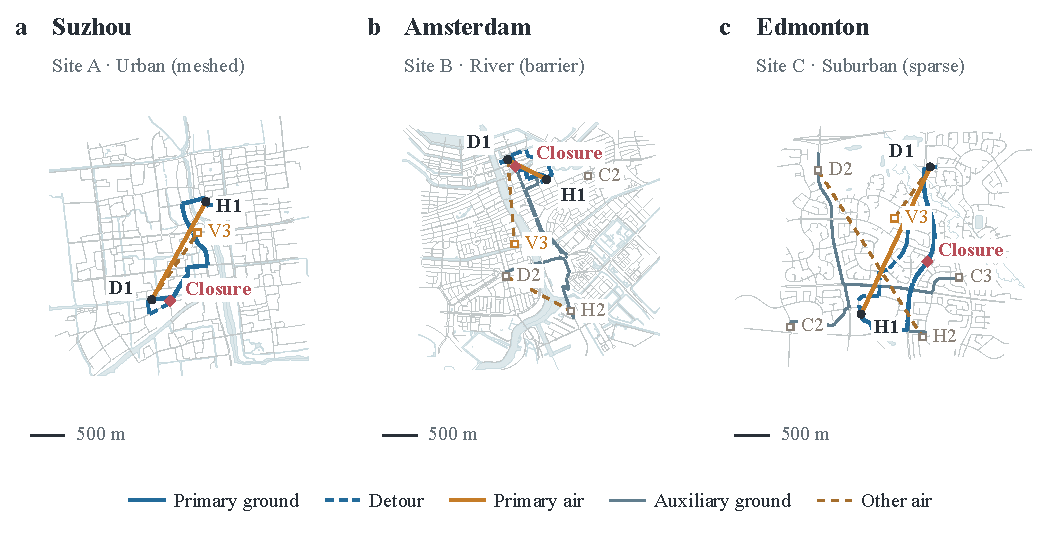
\includegraphics[width=\textwidth]{figures/fig02.pdf}
\caption{Three contrasting network morphology contexts, drawn from archived projected road and facility geometry. Blue indicates the primary ground route and dashed blue the detour; orange denotes low-altitude connections. Thin blue-grey routes show auxiliary ground ODs, and muted orange dashed lines show background air connections where present. D1/H1 mark reference endpoints, V3 a backup landing site, and D2/H2/C2/C3 auxiliary facilities. Co-located landing nodes are not labeled separately. Closure marks the reference disrupted road link. Auxiliary routes describe site context, not additional E1 missions. Maps use a common projected scale and 500 m scale bars. Road and water data: \textcopyright{} OpenStreetMap contributors. Facilities, air operations and disturbances are modeled.}
\label{fig:fig02}
\end{figure}

\begin{table}[!htbp]
\centering
\small
\setlength{\tabcolsep}{3pt}
\caption{Network and reference-service descriptors.}
\label{tab:table3}
\begin{tabularx}{\textwidth}{@{}Yrrr@{}}
\toprule
Descriptor & A: Suzhou & B: Amsterdam & C: Edmonton \\
\midrule
Statistical polygon area (km$^2$) & 10.2450 & 10.2361 & 10.2383 \\
Within-boundary road length (km) & 181.934 & 217.946 & 168.410 \\
Within-boundary road density (km/km$^2$) & 17.758 & 21.292 & 16.449 \\
Within-boundary intersection density (km$^{-2}$) & 37.970 & 100.331 & 39.655 \\
Full routing-network nodes & 542 & 1877 & 791 \\
Full directional passenger edges & 1286 & 3514 & 1681 \\
Full-network mean node degree & 2.830 & 2.663 & 2.420 \\
Full-network dead-end ratio & .1845 & .1193 & .2882 \\
Full-network sampled OD circuity & 1.1969 & 1.1409 & 1.4721 \\
D1--H1 network distance (km) & 2.9222 & 1.1192 & 3.4296 \\
D1--H1 Euclidean distance (km) & 1.7403 & .7246 & 2.5285 \\
D1--H1 circuity & 1.6791 & 1.5446 & 1.3564 \\
Reference closure ETA increase (\%) & 37.87 & 88.69 & 34.76 \\
\bottomrule
\end{tabularx}
\end{table}

Road length is the sum of directional passenger-edge lengths apportioned by the fraction of each polyline inside the configured study polygon. Both density denominators use that polygon's projected area, approximately 10.24 km$^2$. Intersection counts include only nodes inside it, with at least three distinct neighbors in the full graph. The full routing network retains outside roads; its topology and fixed 200-pair OD sample are explicitly labeled separately. D1--H1 quantities describe the reference service pair. Supplementary Section S4 gives the boundary correction.

The sites provide contrasting operating contexts. At Site A, the meshed urban network leaves meaningful choices between continued ground service and reassignment of occupied aircraft. Site B has the highest within-boundary road density, but water barriers constrain its reference ground corridor. Site C has a higher dead-end ratio and mean sampled OD circuity, together with a longer reference service distance. These features provide different transport alternatives. Section 7 discusses why their individual causal effects cannot be separated here.

Every site uses a four-aircraft core fleet: two medical UAVs, one logistics UAV and one passenger eVTOL. Compatibility rules restrict which aircraft can serve each mission. Under low medical workload, the medical aircraft are idle; under high workload, they are assigned to existing services. Facilities, aircraft operations, landing sites and failures are scenario constructs. The experiments thus represent modeled services on real road networks.

\subsection{Shared controls and site adaptations}

Within each experiment, policies share mission semantics, the action contract, candidate-generation rules and deterministic execution constraints. The prompt and B2 objective remain as specified. Across sites, geographic coordinates, road alternatives, aircraft travel distances and failure placement vary. Fault times are adapted to intercept the modeled air operation; an identical time would affect different flight phases. The cross-site evaluation therefore tests the same supervisory architecture in different network and service contexts.

Two comparisons must be distinguished. B0 versus a coordinated policy measures the total difference associated with allowing cross-modal support, including a difference in available transport modes. B1 versus B2 versus B4b compares supervisory implementations under common information and action constraints. In contrast, B4a versus B4b tests explicit candidate presentation within the same LLM implementation. These comparisons answer different questions and are not combined into one ranking of algorithmic intelligence.

\subsection{Disturbance experiments}

\begin{table}[!htbp]
\centering
\small
\setlength{\tabcolsep}{3pt}
\caption{Experiment design and sample sizes. Each primary scenario--arm--policy cell contains 20 paired seeds.}
\label{tab:table4}
\begin{tabularx}{\textwidth}{@{}YYYrr@{}}
\toprule
Experiment & Factors & Sites & Primary runs & Additional B4a runs \\
\midrule
E1 & 3 ground disruption levels $\times$ 2 urgency levels $\times$ 2 workloads & A, B, C & 2,880 & 180 \\
E2 & 16 feasible failure-family/context combinations & A, B, C & 3,840 & 0 \\
E3 v2 & 12 scenarios across four disturbance/task levels & A, B, C & 2,880 & 0 \\
E4A & Observation intervals of 10, 30, 60, 120, 300 s & A & 400 & 0 \\
E4B & Execution delays of 0, 1, 5, 10, 20, 30, 60 s & A & 560 & 0 \\
E4C & Total aircraft records of 5, 10, 20, 30, 50 & A & 400 & 0 \\
\textbf{Total} &  &  & \textbf{10,960} & \textbf{180} \\
\bottomrule
\end{tabularx}
\end{table}

\textbf{E1: ground disruption and selective support.} A new blood-transport mission and a ground disruption occur at 300 s. Ground disruption has three levels, urgency has HIGH and CRITICAL levels, and medical workload is low or high. HIGH urgency has 300 s of deadline slack and CRITICAL urgency has 180 s. The resulting 12 scenarios run for 900 s. Six scenarios per site provide the interface ablation, with ten matched seeds each. The 180 extra runs are B4a runs; their B4b counterparts belong to the primary cohort.

\textbf{E2: individual air-system failures.} The primary CRITICAL mission is released at 300 s and has deadline 480 s. Six failure families model command-and-control link loss, GNSS degradation, UTM degradation/outage, landing-site failure, unknown-aircraft intrusion and flyaway behavior with a moving risk envelope. Context C1 affects a peripheral part of the operation, C2 interrupts the primary service chain while retaining another air option, and C3 removes the relevant air alternatives. F3--C2 and F4--C2 are excluded because the specified mechanisms cannot create the intended combination of interruption and surviving air alternative. The resulting 16 scenarios use fault times of 360, 322 and 383 s at A, B and C, respectively.

\textbf{E3: compound disturbance and competing services.} Twelve scenarios form four levels. L1 comprises two single-failure, single-emergency anchors. L2 comprises four two-failure, single-emergency cascades. L3 comprises four single-failure scenarios with two simultaneous emergency missions and tighter medical-resource availability. L4 comprises two scenarios with multiple emergencies and two or three failures. In the two-emergency scenarios, the second medical mission is released at 300 s with HIGH priority and 240 s of deadline slack. The primary CRITICAL and secondary HIGH missions have delay penalties of 60 and 45 and cancellation penalties of 600 and 450, respectively. Horizons are 900 s for L1/L2 and 1,200 s for L3/L4. These levels change both disturbance structure and task demand and are not a one-dimensional ladder of difficulty.

\subsection{Observation, execution delay and input burden}

E4 retains Site A's core task and examines three operational changes separately. E4A varies the interval between observed snapshots, with a fault at 371 s. Scheduled polling continues throughout the observation experiment, including after some transport decisions have resolved. E4B applies the same specified delay from decision to execution to every policy, with a fault at 360 s. E4C adds unavailable, non-commandable aircraft records with zero endurance and incompatible landing capabilities. It also adds inert facility records and records of completed missions.

E4C keeps the core fleet at four aircraft and adds no usable transport capacity. Candidate invariance is checked at matched decision stages. It tests how added input affects the burden on the policy and its choices for a fixed transport decision. It does not test scheduling fifty operational aircraft or serving a proportionally larger set of urgent missions.

\subsection{Outcomes, pairing and statistical interpretation}

The primary seeds are 20240601--20240620. Each controls the SUMO random seed and a common initial-state realization, including progress and endurance perturbations for aircraft. Busy-aircraft progress is sampled along its route, and remaining endurance receives a seed-dependent reduction of up to 15\%. Comparisons pair policies by scenario and seed. Some outcomes are constant within a cell because the perturbations do not change the executed action or resulting completion time.

Emergency completion and deadline violation follow Equation (7). Existing-service damage counts non-primary missions in state INTERRUPTED, NEEDS\_REPLAN, CANCELLED or FAILED at the horizon. It describes their final service status, not physical damage or the cumulative history of interruptions. Air intervention is identified from issued actions; rejected proposals do not count.

For recovery, let $A_i=1$ if a run's primary air chain is actually affected and $R_i=1$ if an executable replacement service is established. Conditional path restoration is

\begin{equation*}
\widehat P_{\mathrm{rec}}=\frac{\sum_i A_iR_i}{\sum_i A_i}. \tag{10}
\end{equation*}

When no run is affected, the result is N/A. Pairwise recovery-time comparisons include only pairs in which both policies are affected. Completion and deadline comparisons retain all matched runs. Failure-to-replan latency uses the first issued mission-specific DISPATCH, REASSIGN, DIVERT, REROUTE or GROUND\_FALLBACK action after the fault, excluding NO\_ACTION. Path restoration and completed transport are separate events.

E3's system weighted loss (SWL) is

\begin{equation*}
L_H=\sum_{m\in M_H}w_{p_m}\ell_m(H),\qquad
w_{\mathrm{CRITICAL,HIGH,NORMAL,LOW}}=(4,3,2,1), \tag{11}
\end{equation*}

with

\begin{equation*}
\begin{aligned}
\ell_m(H)&=\begin{cases}
q_m^{\mathrm{delay}},&m\text{ completed and }c_m>d_m,\\
q_m^{\mathrm{cancel}},&\operatorname{state}_m(H)\in\mathcal U,\\
0,&\text{otherwise},
\end{cases}
\\[4pt]
\mathcal U&=\{\mathrm{CANCELLED,FAILED,INTERRUPTED},
\\&\qquad\mathrm{NEEDS\_REPLAN,WAITING}\}.
\end{aligned}\tag{12}
\end{equation*}

Late completion incurs a fixed penalty, not a charge per second late. EN\_ROUTE and ASSIGNED services incur no horizon penalty. The terminal-registry audit found that all 4,320 E3 task instances with deadlines at or before the horizon had completed. No overdue ongoing tasks were therefore omitted. A late primary CRITICAL mission contributes 240 units, and a late secondary HIGH mission contributes 135 units. SWL uses configured loss units rather than monetary welfare. We also report its CRITICAL+HIGH component for compound-level policy comparisons.

The estimand is defined over the fixed scenario panel. Scenario--seed runs receive equal weight, preserving E3 level sample sizes of 40, 80, 80 and 40 per policy. For each scenario, initialization restarts \nolinkurl{random.Random(seed)}, visits aircraft in sorted order and passes the same seed to SUMO. Workload can change the number of random draws, but it does not create independent scenario streams. We therefore estimate uncertainty by grouping the complete fixed panel by seed, with policies paired within each scenario and seed.

For a complete panel with $J$ scenarios and $K$ seeds, define
\begin{equation*}
D_s=\frac{1}{J}\sum_{j=1}^J(Y^{(u)}_{js}-Y^{(v)}_{js}),\qquad
\overline D=\frac1K\sum_sD_s,\qquad
\mathrm{CI}_{95\%}=\overline D\pm t_{0.975,K-1}\frac{s_D}{\sqrt K}.\tag{13}
\end{equation*}

Primary panels use $K=20$; the six-scenario E1 ablation uses $K=10$. Means and scenario weights are unchanged by blocking. Continuous comparisons use a paired t test on seed aggregates, with the previously specified signed-rank fallback for constant nonzero differences. Identical differences receive $p=1$. Binary comparisons swap policy labels for entire seed blocks in an exact paired randomization test, preserving within-seed dependence. This replaces run-independent McNemar inference for multi-scenario panels. Unadjusted intervals describe fixed-panel seed uncertainty; a zero-width interval means no variation across these seed aggregates. Supplementary Section S3 specifies the conditional-denominator calculation and provides the complete revised tests.

Holm adjustment retains the original comparison families: three E1 ablation endpoints per site; 12 scenario-specific E1 completion tests; 12 E2 endpoints per site; and 12 E3 compound comparisons per site. E4 retains separate per-policy, per-metric non-anchor comparisons with OBS30, D00 and N05. Adjusted $p<0.05$ is the decision criterion. \citep{ref18} The sites form separate fixed transport contexts, and nonsignificance is not statistical equivalence.

\subsection{Provenance and model scope}

The experiments evaluate supervisory service replacement with four core aircraft, specified fault state machines and the ground timer described in Section 4.1. External inference calls do not advance physical simulation time. E4A changes the information observed by the supervisor; E4B inserts a controlled wait before execution. Backend wall-clock latency is recorded separately. The numerical revision retains the original runs, corrects the B0 D60 duplicate-command cell through a local implementation overlay, and recalculates fixed-panel statistics. The supplementary materials provide parameters, prompts, analysis scripts and revision provenance.

\section{Results}

\subsection{Selective air support and incumbent-service cost}

Air support improved emergency transport, but the coordinated policies differed in how much incumbent service they disrupted (Figure~\ref{fig:fig03}). At A, B2 and B4b reduced deadline violations from B0's 33.33\% to 16.67\%. Their mean completion durations were 147.62 and 146.63 s, respectively. However, B4b left 0.133 damaged services per run, compared with B2's 0.058. Supplementary Table S1 provides the full site--policy summaries and intervals.

\begin{figure}[!htbp]
\centering
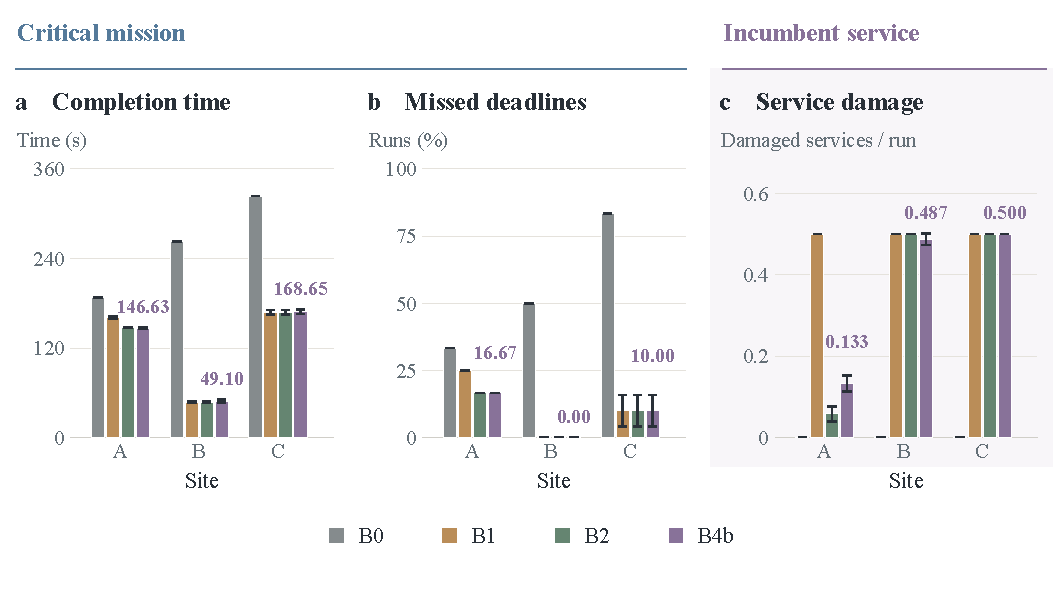
\includegraphics[width=\textwidth]{figures/fig03.pdf}
\caption{E1 service benefit and incumbent cost. Clustered bars show site--policy mean completion time, missed deadlines and incumbent services damaged at the horizon. Whiskers are 95\% seed-block intervals (240 runs, 20 seed blocks per site and policy). All bars start at zero; zero-width intervals have coincident caps. Colors identify policies consistently across the result figures. Labels above B4b bars show completion time and missed deadlines to two decimals and incumbent damage to three decimals. Supplementary Table S1 retains exact values.}
\label{fig:fig03}
\end{figure}

The high-disruption, HIGH-urgency, high-workload scenario at A shows what this trade-off means for service. Ground transport could meet the 300 s deadline slack, and B2 selected it in all 20 runs. B4b reassigned an occupied aircraft in 12 runs and used ground in eight. Relative to B2, completion duration decreased by 11.95 s (95\% CI -17.330 to -6.570; Holm-adjusted $p=0.002100$), while damage increased by 0.600 services per run. Both policies met every emergency deadline. Air reassignment therefore accelerated the emergency by interrupting another service, even though ground could still finish on time. An operator must weigh that interruption against the additional speed.

At B and C, coordinated policies achieved large gains over ground-only operation but produced similar outcomes to one another. Their deadline-violation rates were 0\% and 10\%, respectively, compared with B0's 50.00\% and 83.33\%. These results separate the benefit of allowing a useful transport mode from the effect of choosing a more complex supervisor.

\subsection{The candidate interface shapes supervisory choices}

Explicit candidate-information support improved speed and preserved more incumbent service at A (Table 5). Relative to B4a, B4b reduced completion duration by 13.567 s, damage by 0.383 services per run and air intervention by 38.333 percentage points. Improving all three outcomes indicates more selective use of the same transport resources.

\begin{figure}[!htbp]
\centering
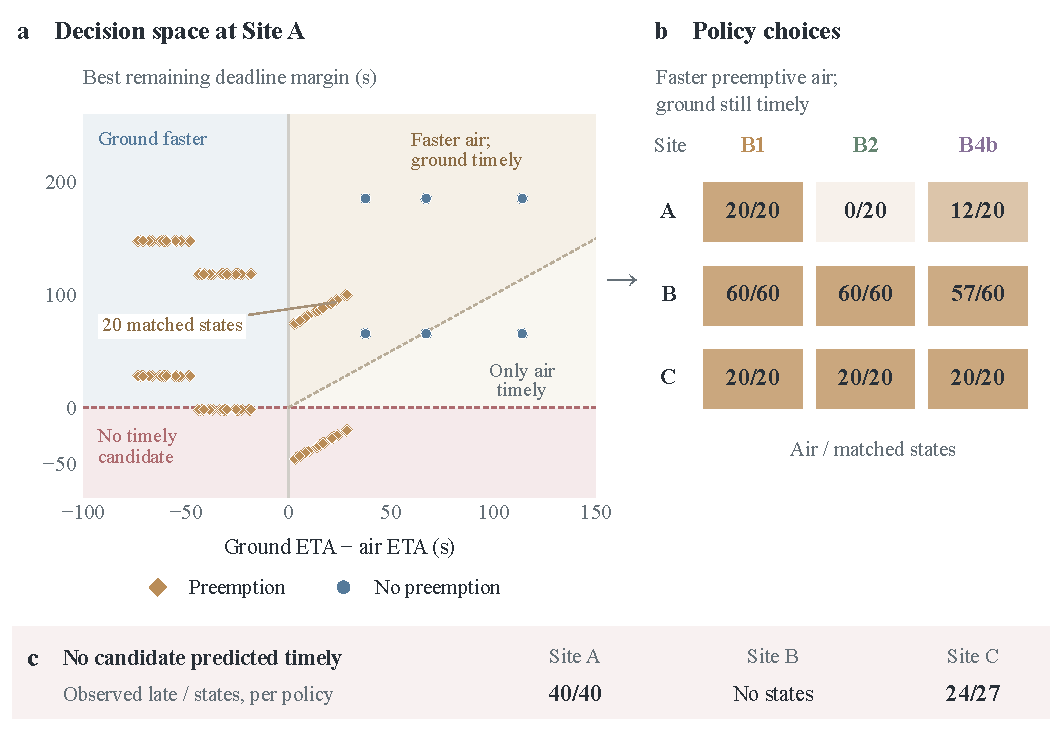
\includegraphics[width=\textwidth]{figures/fig04.pdf}
\caption{Supervisory decision regimes from E1 first-decision logs. (a) Site A candidate geometry relates the air ETA advantage to the best remaining deadline margin; symbols distinguish preemption. Repeated locations represent multiple matched states. Pale regions distinguish predicted timing conditions. When air is faster, the diagonal marks zero predicted ground margin. (b) Matrix cells show air selections divided by matched states when faster air requires preemption and ground remains timely, with 20, 60 and 20 states at A, B and C. Darker cells indicate a larger selected fraction. (c) Among states with no candidate predicted timely, observed late counts are 40/40 at A and 24/27 at C per policy; B has no such states. First candidate snapshots match across B1, B2 and B4b in all 720 scenario--seed states. Subsequent actions and trajectories may differ. ETA-based groups are descriptive, not a new policy score.}
\label{fig:fig04}
\end{figure}

\begin{table}[!htbp]
\centering
\small
\setlength{\tabcolsep}{3pt}
\caption{Paired E1 interface ablation: B4b minus B4a.}
\label{tab:table5}
\begin{tabularx}{\textwidth}{@{}lYrYYY@{}}
\toprule
Site & Endpoint & Pairs & Difference & 95\% seed-block interval & Holm p \\
\midrule
A & Completion (s) & 60 & -13.567 & [-15.978, -11.155] & 9.33e-07 \\
A & Damaged services/run & 60 & -0.383 & [-0.441, -0.326] & 3.27e-07 \\
A & Air intervention (pp) & 60 & -38.333 & [-44.093, -32.574] & 0.001953 \\
B & Completion (s) & 60 & 1.450 & [-2.288, 5.188] & 1.000 \\
B & Damaged services/run & 60 & -0.017 & [-0.054, 0.021] & 1.000 \\
B & Air intervention (pp) & 60 & -1.667 & [-5.437, 2.104] & 1.000 \\
C & Completion (s) & 60 & 0.000 & [0.000, 0.000] & 1.000 \\
C & Damaged services/run & 60 & 0.000 & [0.000, 0.000] & 1.000 \\
C & Air intervention (pp) & 60 & 0.000 & [0.000, 0.000] & 1.000 \\
\bottomrule
\end{tabularx}
\end{table}

Each site retains a three-endpoint adjustment family. Intervals use ten seed blocks; air intervention is a risk difference in percentage points (pp) with exact whole-block label-swap inference.

The effect of information support differed by site. At B, no difference passed Holm adjustment; at C, all three endpoint differences were zero. Figure~\ref{fig:fig04} relates choices to ETA advantage, deadline margin and preemption. When ground is faster and avoids preemption, it is preferable on both service criteria. B1 can still select air because its rule ranks only air candidates. Available candidates therefore do not by themselves ensure a useful choice.

At A, 20 states offered faster air requiring preemption and ground that could still meet the deadline. B1, B2 and B4b selected air in 20, zero and 12 cases, respectively. The corresponding counts at B and C were 60/60/57 and 20/20/20. Thus, a conflict between speed and incumbent service did not always lead policies to choose differently.

When A had no candidate predicted to finish on time, all 40 runs per coordinated policy were late despite different mode choices. At C, 24 of 27 such cases were late. The three timely cases show that candidate ETA is approximate. These observations link explicit information support to policy decisions while distinguishing predicted deadline margins from guaranteed completion.

\subsection{Restored paths do not guarantee timely recovery}

Every affected coordinated run established an executable replacement path in E2 (Supplementary Figure S1). Earlier assignments changed exposure to failure, so B4b had different affected counts from B1/B2; B0's conditional recovery was N/A. Despite restoration in every affected run, B4b's deadline-violation rates over all runs remained 39.06\%, 37.50\% and 62.81\% at A, B and C. Traveling along a surviving route could require more time than remained before the deadline.

At A, B4b completed later than B2, and the difference passed the specified multiplicity-adjusted test (Table 6). The conditional recovery-time difference did not pass correction. Completion differences at B and C were smaller and did not pass Holm adjustment. Establishing a replacement service quickly does not eliminate the travel time remaining after a fault. Dispatch latency and deadline performance therefore describe different operational outcomes.

\begin{table}[!htbp]
\centering
\small
\setlength{\tabcolsep}{3pt}
\caption{Selected E2 paired comparisons: B4b minus B2.}
\label{tab:table6}
\begin{tabularx}{\textwidth}{@{}lYrYYY@{}}
\toprule
Site & Endpoint & Pairs & Difference & 95\% seed-block interval & Holm p \\
\midrule
A & Completion (s) & 320 & 4.525 & [2.412, 6.638] & 0.003069 \\
A & Recovery time (s) & 191 & 3.927 & [0.930, 6.924] & 0.142465 \\
B & Completion (s) & 320 & 0.175 & [0.060, 0.290] & 0.055710 \\
B & Recovery time (s) & 199 & 0.281 & [0.098, 0.465] & 0.055710 \\
C & Completion (s) & 320 & 0.922 & [-0.214, 2.057] & 1.000 \\
C & Recovery time (s) & 200 & 0.255 & [-0.138, 0.648] & 1.000 \\
\bottomrule
\end{tabularx}
\end{table}

Adjustment uses the original 12-endpoint family per site. Completion uses all matched runs; recovery time uses jointly affected pairs. Intervals are unadjusted and p-values are multiplicity-adjusted. At C, 201 B4b runs were affected but only 200 pairs were jointly affected. Backend errors and retries remain included; some deterministic replacement decisions occur within the fault's simulation second.

\subsection{Compound service loss depends on surviving options}

Coordination reduced aggregate priority-weighted loss in E3 (Figure~\ref{fig:fig06}; Supplementary Tables S3 and S7). At A, SWL fell from 240 under B0 to 100 under B1/B2 and 102.125 under B4b. At B and C, coordinated policies shared aggregate means of 127.5 and 227.5, respectively, against 307.5 under B0.

\begin{figure}[!htbp]
\centering
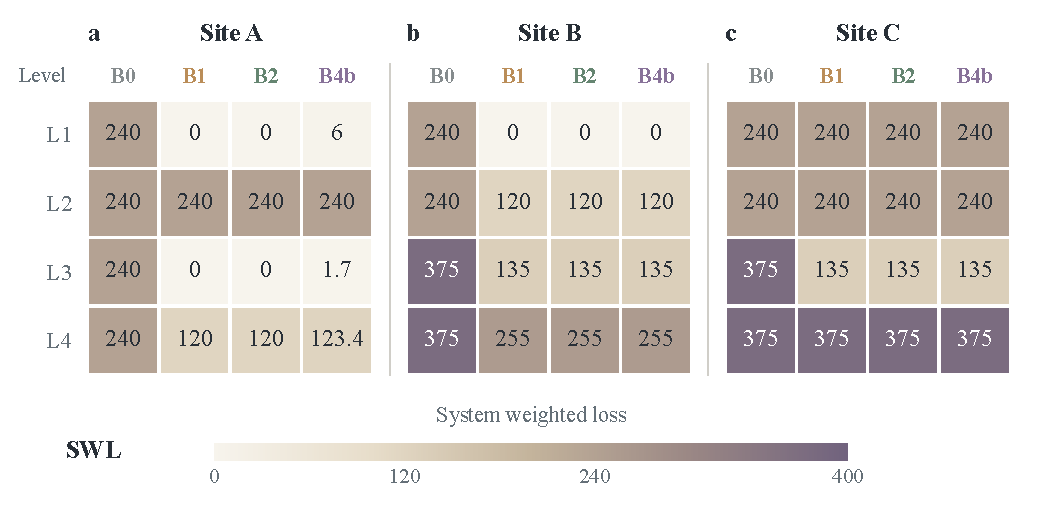
\includegraphics[width=\textwidth]{figures/fig06.pdf}
\caption{E3 service loss across compound settings. (a--c) All policy--level means share one SWL color scale; noninteger labels are rounded to one decimal. Each policy has 40 runs in L1/L4 and 80 in L2/L3. Levels jointly vary disturbance and demand. Supplementary Figure S3 shows paired B4b-minus-B0 differences and 95\% seed-block intervals; negative values indicate lower loss under B4b. Exact values remain in Supplementary Tables S3 and S7.}
\label{fig:fig06}
\end{figure}

Coordination did not reduce loss in every setting. At A, all policies retained loss 240 in L2. At C, coordination reduced SWL only in L3, with no reduction in L1, L2 or L4. The E1 benefit of air availability therefore did not persist across every combination of failures and service demand.

B4b did not significantly reduce SWL or CRITICAL+HIGH loss relative to B1 or B2 in the recorded compound comparison families. At A, its L3 and L4 SWL differences were +1.6875 (95\% CI [-1.844, 5.219]) and +3.375 ([-3.689, 10.439]), with adjusted $p=1$. The corresponding compound-level differences at B and C were zero. In these panels, surviving alternatives that could meet deadlines accounted for the transport benefit; differences between policies added little protection.

Mean primary completion time did not capture all service benefits. At A, coordinated policies reduced SWL even though mean primary completion took longer than under B0. The configured loss depends on which priority-weighted services miss their deadlines, not only on how quickly the primary mission finishes on average.

\subsection{Contrasting morphology and policy sensitivity}

The sites show that an opportunity for coordination need not imply strong sensitivity to policy choice. At A, ground can remain timely while air reassignment offers a smaller speed gain at the cost of incumbent service. This site also has the strongest interface effect. B combines a dense network with a barrier-constrained reference corridor. C has more dead ends, higher sampled OD circuity and a longer reference trip. Both have large E1 coordination benefits and similar outcomes across coordinated policies.

C's limited E3 gains show the boundary of this pattern: an alternative must meet the relevant deadline to avoid the configured penalty. Road geometry, facilities, air travel times and fault timing vary together across sites. Morphology helps explain the context in which the supervisor chooses; the comparison does not estimate an independent causal effect of density, circuity or redundancy.

\subsection{Timing conditions and input burden}

\subsubsection{Observation scheduling}

Longer observation intervals could leave too little time to complete the service (Figure~\ref{fig:fig07}a; Supplementary Table S4). B2/B4b completion duration increased from 140 s at OBS10 to 482 s at OBS300. Their results matched in every arm. B1 differed at OBS300, completing in 521 s. All B4b runs in OBS10--OBS60 met the deadline, with OBS60 exactly on time; all runs in OBS120/OBS300 were late.

\begin{figure}[!htbp]
\centering
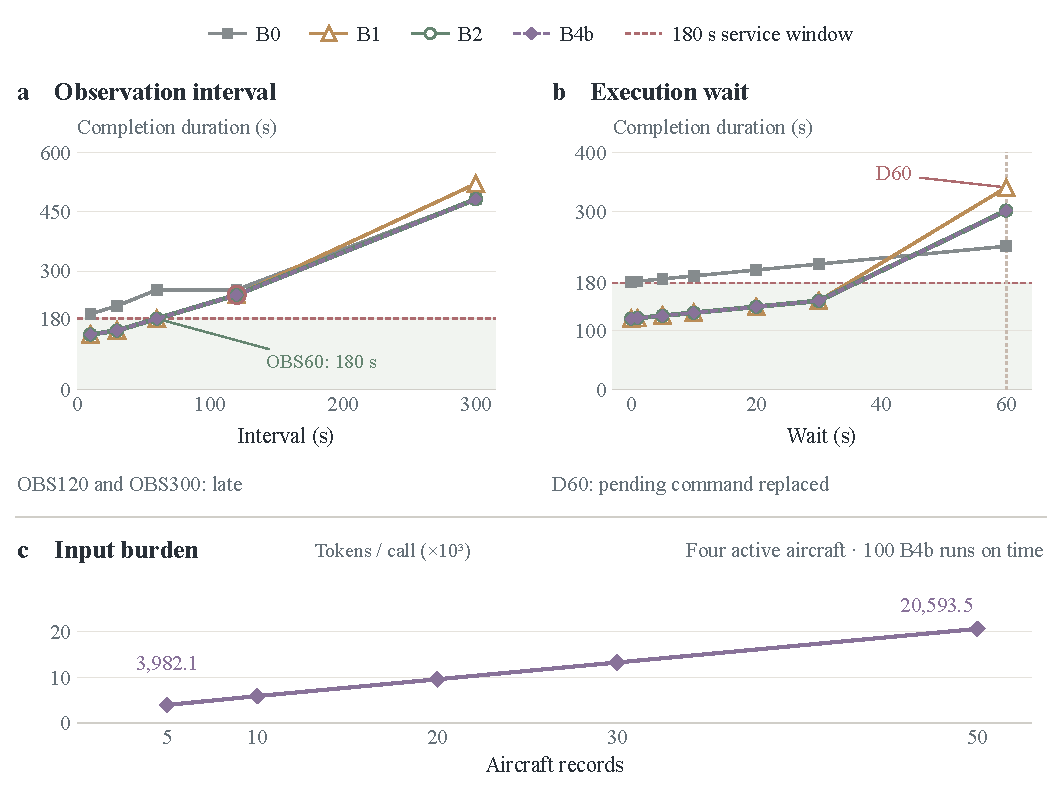
\includegraphics[width=\textwidth]{figures/fig07.pdf}
\caption{E4 timing and input burden at Site A. Panels (a,b) show mean completion duration for 20 runs per arm and policy. The dashed horizontal line marks the 180 s service window; straight segments join measured settings. B2/B4b coincide, as does B1 at 0--30 s in (b); nested markers identify overlapping policies. Panel (c) shows prompt tokens per logged call for 5--50 records around four active aircraft.}
\label{fig:fig07}
\end{figure}

The observation schedule delayed discovery of both the task and the fault. The 300 s snapshot was taken before the task event in the same simulation second. The task first appeared at 310/330/360/360/600 s across the five arms, and the 371 s fault appeared at 380/390/420/480/600 s. OBS120 restored the affected path but completed late. OBS300 had no affected primary air chain, so conditional recovery was N/A. The snapshot timestamp alone therefore did not establish which events were visible.

Longer intervals also reduced B4b decisions from 62 to four per run. These counts cover polling over the fixed full horizon, including calls after some services had resolved. They do not estimate the call count for an adaptive policy that stops polling after completion.

\subsubsection{Execution waiting and command replacement}

Across injected waits of 0--30 s, B1/B2/B4b completion rose from 120 to 150 s and remained timely. At D60, all B4b runs were late, and B1 completed in 341 s (Figure~\ref{fig:fig07}b; Supplementary Table S5).

Identical pending commands retain their original execution time, whereas a changed intervention replaces the previous command. At D60, B0 completes ground service in 242 s. In B2/B4b, replacing the pending air intervention with ground service increases completion to 302 s. The fault at 360 s supersedes the air command selected at 300 s; ground service then executes at 420 s and completes at 602 s. This sequence reflects command replacement rather than rejection of a stale action (Supplementary Section S4.1 and Figure S2).


\subsubsection{Input burden with a fixed active fleet}

Increasing total aircraft records from five to fifty raised B4b prompt tokens per logged call from 3,982.1 to 20,593.5 (Figure~\ref{fig:fig07}c; Supplementary Table S6). The active fleet remained four aircraft. Across 640 matched-stage checks, the legal candidates stayed the same. All 100 B4b runs completed on time, with no observed selection of an illegal or nonexistent resource.

Mean completion duration was 121.5 s in N05 and 120 s in N10--N50. N05 included one retained transport error and another decision opportunity. Across E4, the records contain four final transport-error calls and four structured retries, all retained in the analysis. These results concern input burden for a fixed service problem, not coordination of fifty operational aircraft.

\FloatBarrier
\section{Discussion}

\subsection{An executable service-management architecture}

The Manager provides a service-level supervisory architecture that treats a service intervention as the unit of transport decision-making. A joint state observation becomes useful when the candidate generator links it to a compatible resource, an executable action and an estimated completion time. The candidate interface also shows which incumbent service would be interrupted. With common checking and execution rules, researchers can compare policy preferences under the same transport contract. This extends multimodal recovery and dynamic fleet management to a failure-prone ground--air service system. \citep{ref4,ref20,ref22}

A replaceable policy layer is useful because service choices matter most where feasible alternatives leave room for different preferences. Deterministic and LLM policies often produced similar outcomes when the surviving alternatives constrained what could be achieved. When ground remained timely but faster air required preemption, their choices could differ. B2 values speed and incumbent service through fixed weights; B4b sometimes interrupts an incumbent to complete the emergency faster. By exposing this choice, the Manager lets an operator assess it against service obligations.

\subsection{Useful alternatives and the remaining service margin}

Low-altitude capacity improves resilience when it provides a useful alternative that can be executed in time. E1 shows how air transport can bypass a disruption and what is lost when an occupied aircraft is reassigned. E2 distinguishes path restoration from on-time completion. E3 shows that surviving options can protect priority-weighted services, whereas exhausted alternatives leave the same loss across policies. Together, these findings link network recovery to the service outcomes that justify intervention. \citep{ref1,ref3}

The decision logs help explain when choices converge or diverge. Policies tend to agree when one option is both faster and preserves incumbent service. Smaller speed gains that require preemption reveal their different preferences. Negative predicted margins identify services that are difficult to rescue, but the estimates remain approximate: a few Site C missions finished on time despite negative candidate margins. The interface must therefore show how ETA and service consequences were derived, and readers must assess timing estimates alongside realized trajectories.

The value of low-altitude support therefore depends on the time available across the service chain, including handling and transfer. In the offline E2 analysis, affected timely services at Site B had only 19 s remaining. Adding 30 s to their recorded completion times would make 80 services per coordinated policy late. At Site A, timely B1/B2 replacements retained 60 s, whereas some B4b trajectories were closer to the deadline. In the separate Site A preemption example, an extra 17 s of air-specific handling would erase the realized speed advantage (Supplementary Section S4.2). These results identify where omitted stages could change the benefit of air support.

\subsection{Observation and execution are management decisions}

Observation scheduling determines when the supervisor can see a mission or fault. Queue rules determine whether an accepted intervention executes before circumstances change. E4 shows that sparse observation can leave too little time to meet the deadline, while execution waiting can allow a fault to replace an air command with ground service. A practical Manager therefore needs observations timed to service deadlines and repeat commands that do not restart a pending wait, as well as a capable selection policy.

Explicit candidate information increases the input the policy must process. The B4a--B4b comparison measures the support provided by derived candidate facts, while E4C measures input burden around a fixed active fleet. Together, they suggest that interface design and policy selection should be considered jointly. The interface should make consequential service choices easy to compare without burying them among unnecessary records.

\subsection{Scope and next steps}

The experiments evaluate supervisory choices under modeled service rules. Ground fallback uses a corridor ETA timer without dispatching a separate road vehicle for each service. The registry does not track payload custody or synchronized physical transfer, and the offline added-time analysis holds subsequent decisions fixed. Benefits in physical deployment remain untested.

The evidence comes from fixed, site-adapted scenario panels with a four-aircraft core fleet. Road morphology varies together with facility placement, flight distance and fault timing, limiting what can be attributed to geometry alone. Faults and feasibility checks follow specified service-level rules. SWL uses configured flat penalties; incumbent damage counts final states. The LLM results concern one recorded backend and prompt family, with wall-clock inference decoupled from simulated transport.

To estimate deployment benefits, future tests should represent task-specific ground travel and explicit payload transfer, allowing handling delays to change later decisions in the closed loop. Larger active fleets and controlled changes in transport geometry would test how far the observed mechanisms generalize to other operating conditions.

\section{Conclusions}

The Manager connects joint transport observations to executable service reconfiguration. Its shared candidate interface lets replaceable supervisory policies compare feasibility, remaining time and consequences for incumbent services. The closed-loop experiments show when selective air support helps, when faster emergency transport costs incumbent service, and why restoring a path does not guarantee timely recovery.

Low-altitude capacity alone does not ensure resilience. It is useful when the supervisor selects a suitable cross-modal intervention and the executor applies it before the remaining service margin runs out. Surviving alternatives determine which services can be rescued. Policy preferences determine whether additional emergency speed justifies interrupting an incumbent service, and observation--execution timing determines whether the selected intervention takes effect. The Manager provides a concrete architecture and comparative evidence for managing these dependencies.

\section*{Data and code availability}
The accompanying research package contains run artifacts, experiment configurations, prompt files, analysis scripts, revised figure data and an executable queue-correction overlay. Supplementary Section S6 identifies the files and reproduction commands. All data and code are publicly available in the GitHub repository: AnXu-ITS/global-llm-mobility-reconfiguration.

\bibliographystyle{tfcad}
\bibliography{references}
\end{document}
